%-------------------------
% Resume in Latex
% Author : Javier Tarazona
%------------------------

\documentclass[letterpaper,10pt]{article}
\DeclareUnicodeCharacter{00A0}{~}
\DeclareUnicodeCharacter{2013}{\textendash}
\DeclareUnicodeCharacter{2014}{\textemdash}
\DeclareUnicodeCharacter{201C}{``}
\DeclareUnicodeCharacter{201D}{''}
\DeclareUnicodeCharacter{2022}{\textbullet}
\DeclareUnicodeCharacter{25E6}{\textopenbullet}
% \setlist[itemize]{label=\textbullet, labelsep=0.5em, leftmargin=*} % Moved after \begin{document}
\usepackage[T1]{fontenc}      % Codificación de salida (acentos y símbolos)
\usepackage[empty]{fullpage}
\usepackage[export]{adjustbox}
\usepackage[pdftex]{hyperref}
\usepackage[usenames,dvipsnames]{color}
\usepackage[utf8]{inputenc}   % Lee texto en UTF-8
\usepackage{array}
\usepackage{comment}
\usepackage{enumitem}
\usepackage{enumitem}         % Control de listas (si no lo tienes ya)
\usepackage{fancyhdr}
\usepackage{graphicx}
\usepackage{latexsym}
\usepackage{lmodern}
\usepackage{marvosym}
\usepackage{tabularx}
\usepackage{titlesec}
\usepackage{verbatim}
\usepackage{xcolor}


\usepackage{latexsym}
\usepackage[empty]{fullpage}
\usepackage{titlesec}
\usepackage{marvosym}
\usepackage[usenames,dvipsnames]{color}
\usepackage{verbatim}
\usepackage{enumitem}
\usepackage[pdftex]{hyperref}
\usepackage{fancyhdr}
\usepackage{tabularx}
\usepackage{graphicx}
\usepackage{array}
\usepackage[export]{adjustbox}
\usepackage{xcolor}
\usepackage{comment}

\begin{comment}  
\end{comment}
% --- Codificación y fuentes seguras ---
\usepackage[utf8]{inputenc}   % Lee texto en UTF-8
\usepackage[T1]{fontenc}      % Codificación de salida (acentos y símbolos)
\usepackage{enumitem}         % Control de listas (si no lo tienes ya)

% --- Viñetas limpias y seguras ---
\setlist[itemize]{label=\textbullet, labelsep=0.5em, leftmargin=*}
%\end{comment}

\pagestyle{empty}

% Adjust margins
\addtolength{\oddsidemargin}{-0.45in}
\addtolength{\evensidemargin}{-0.45in}
\addtolength{\textwidth}{1.15in}
\addtolength{\topmargin}{-.62in}
\addtolength{\textheight}{1.20in}

\urlstyle{same}

\raggedbottom
\raggedright
\setlength{\tabcolsep}{0in}
\renewcommand{\arraystretch}{0.98}

%\definecolor{mydarkgreen}{RGB}{0, 140, 123}
\definecolor{mydarkgreen}{RGB}{0, 0, 0}

% Sections formatting
\titleformat{\section}{
  \vspace{-5pt}\scshape\raggedright\large
}{}{0em}{}[\color{mydarkgreen}\titlerule \vspace{-6pt}]

%-------------------------
% Custom commands
\newcommand{\resumeItemCompact}[2]{\item\small{\textbf{#1}: #2}\vspace{-2pt}}
\newcommand{\resumeItemListStartCompact}{\begin{itemize}[leftmargin=*,itemsep=0pt,parsep=0pt,topsep=0pt,partopsep=0pt,nolistsep]}
\newcommand{\resumeItemListEndCompact}{\end{itemize}\vspace{-4pt}}

\newcommand{\resumeItem}[2]{
  \item\small{
    \textbf{#1}{: #2 \vspace{-2pt}}
  }
}

\newcommand{\resumeSubheading}[4]{
  \vspace{-1pt}\item
    \begin{tabular*}{0.97\textwidth}{l@{\extracolsep{\fill}}r}
      	\textbf{#1} & \textbf{\textcolor{mydarkgreen}{#2}} \\
      	\textit{\footnotesize#3} & \textit{\footnotesize \textcolor{mydarkgreen}{#4}} \\
    \end{tabular*}\vspace{-4pt}
}

\newcommand{\resumeSubItem}[2]{\resumeItem{#1}{#2}\vspace{-4pt}}

\renewcommand{\labelitemii}{$\circ$}

\newcommand{\resumeSubHeadingListStart}{\begin{itemize}[leftmargin=*]}
\newcommand{\resumeSubHeadingListEnd}{\end{itemize}}
\newcommand{\resumeItemListStart}{\begin{itemize}[itemsep=0pt,parsep=0pt,topsep=0pt,partopsep=0pt]}
\newcommand{\resumeItemListEnd}{\end{itemize}\vspace{-5pt}}

% Indented paragraph helper: \indentbox[ancho]{contenido}
% Uso: \indentbox{Texto...}  o  \indentbox[1.5em]{Texto...}
\newcommand{\indentbox}[2][1em]{\hspace*{#1}\parbox{\dimexpr\linewidth-#1\relax}{#2}}

\newlength{\headerPhotoSpace}
\setlength{\headerPhotoSpace}{0pt}
\newcommand{\showHeaderPhoto}{%
  \setlength{\headerPhotoSpace}{0.13\textwidth}%
  \makebox[0pt][l]{\adjustbox{valign=c}{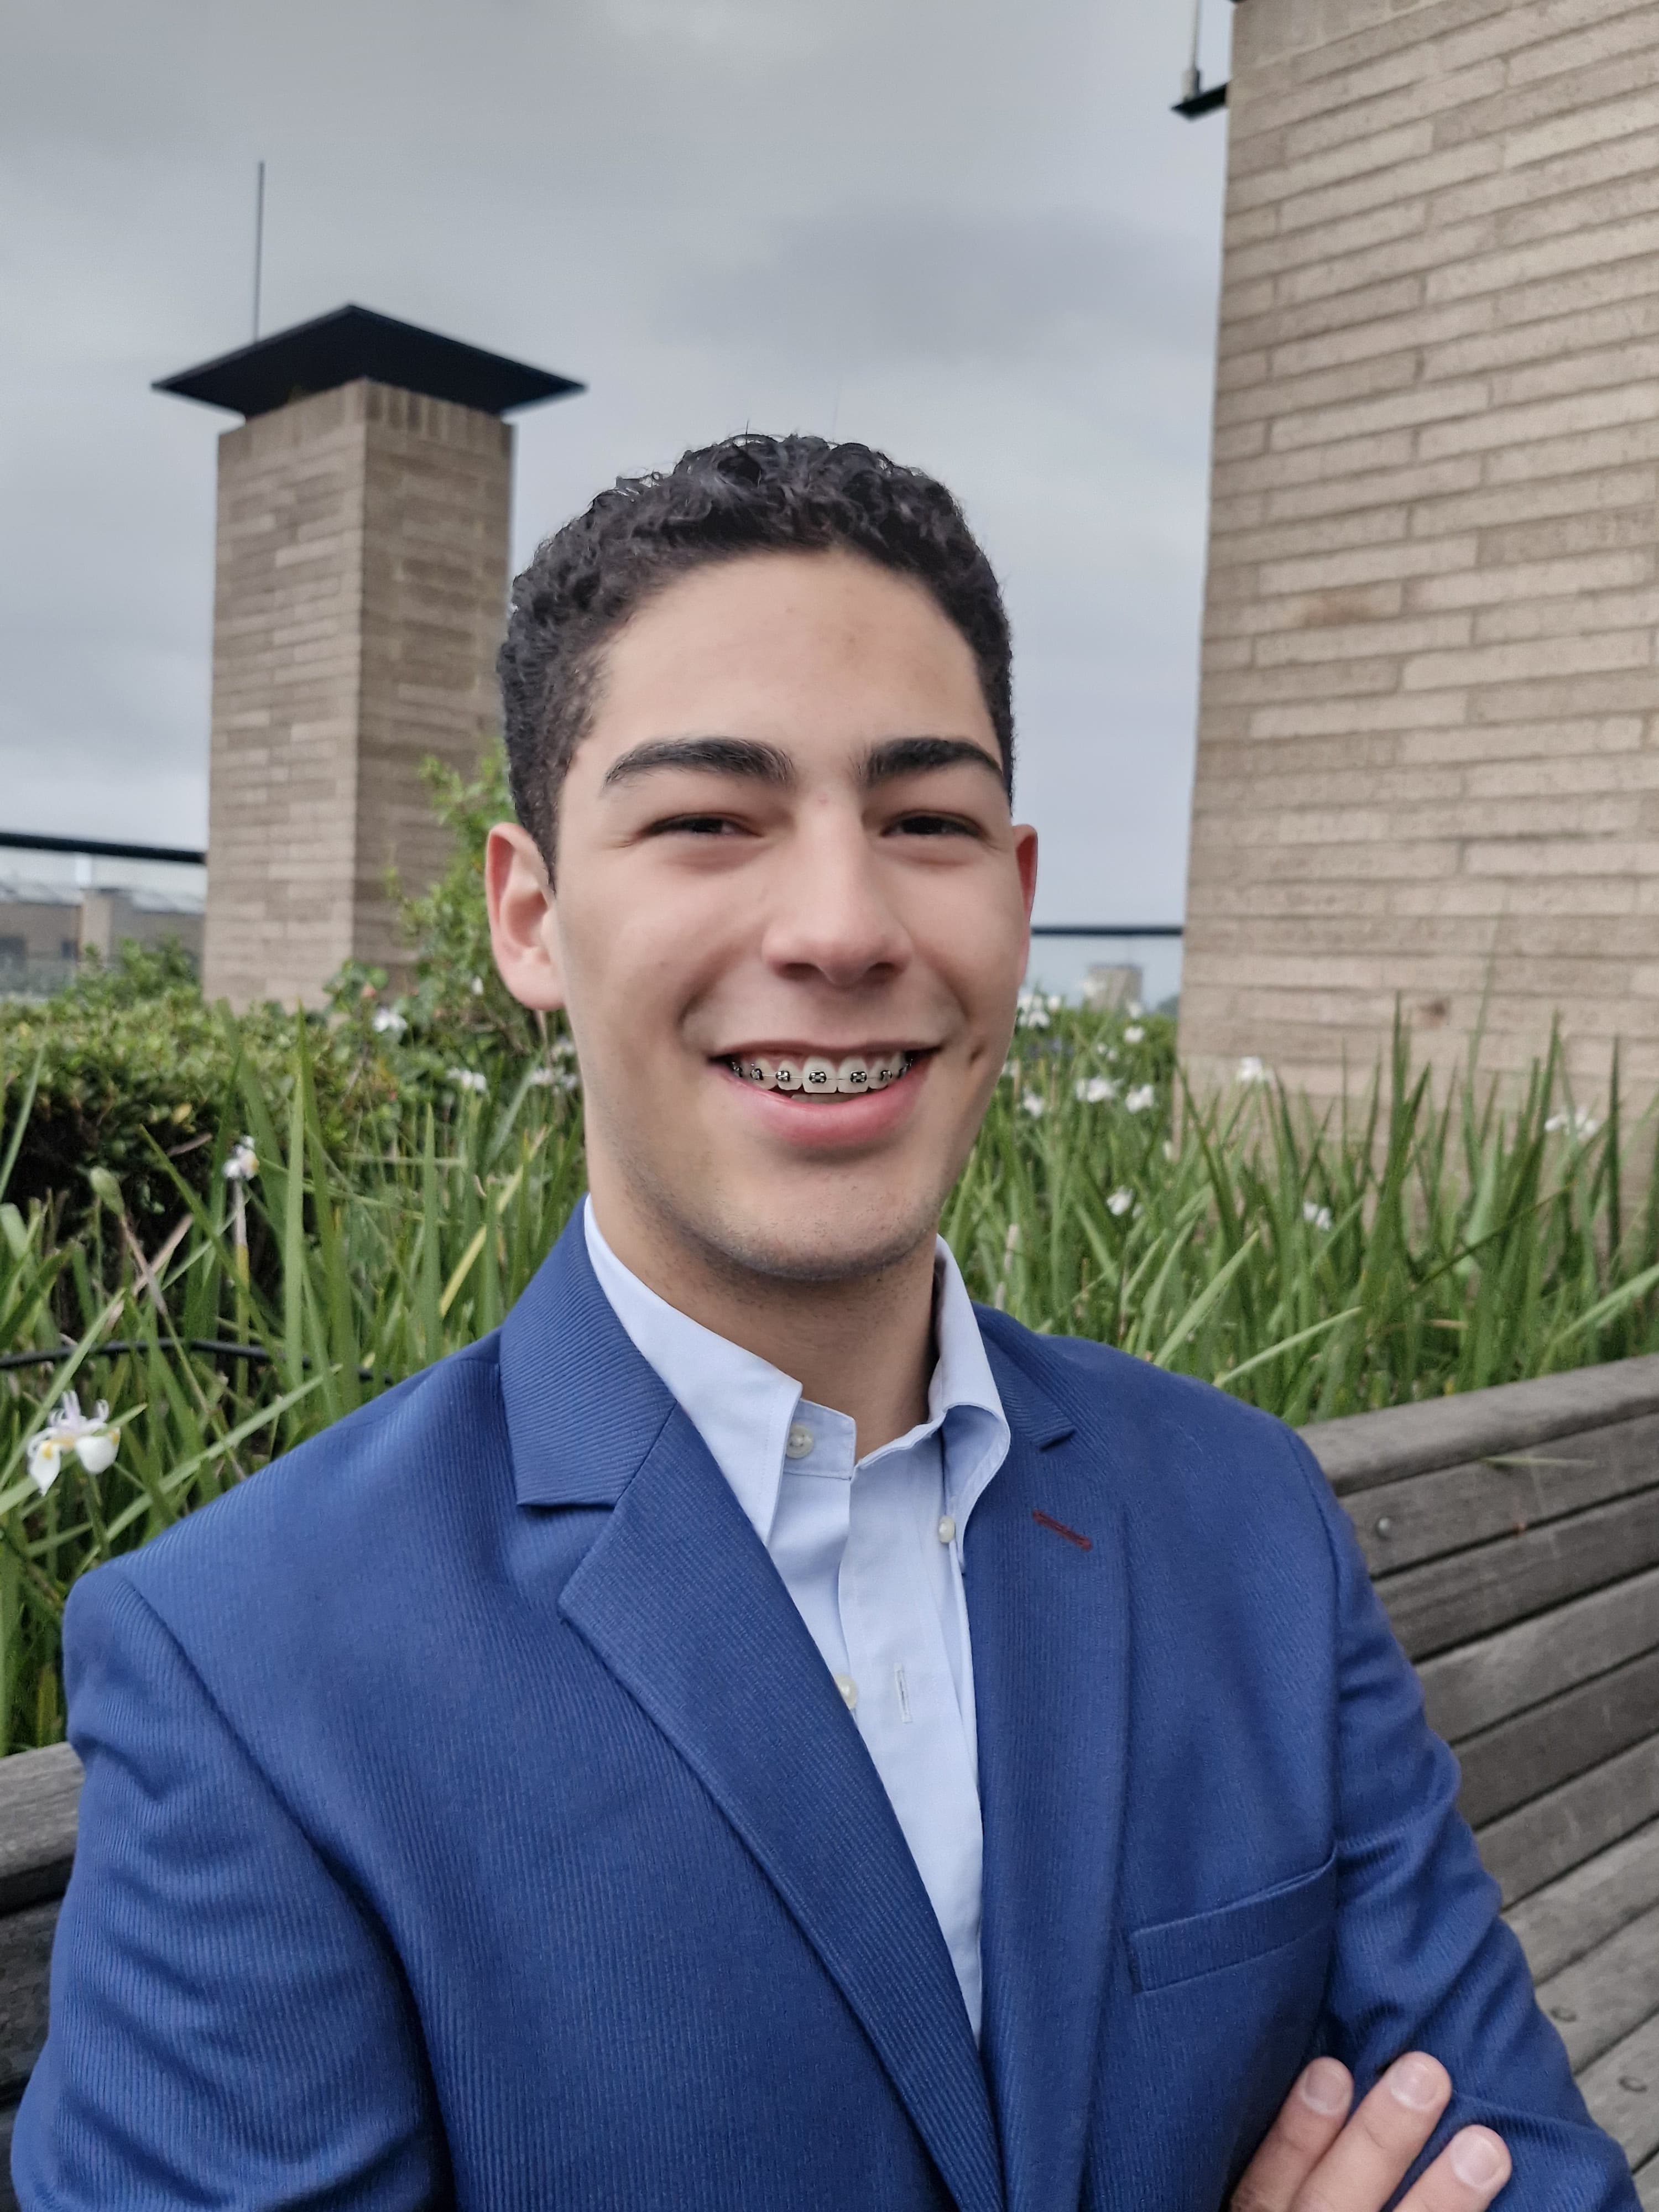
\includegraphics[scale=0.015]{../fr/Digital_photo.jpg}}}%
}


%-------------------------------------------
%%%%%%  CV STARTS HERE  %%%%%%%%%%%%%%%%%%%%%%%%%%%%


\begin{document}

\begin{comment}
\AddToHookNext{shipout/foreground}{%
  \put(\dimexpr\paperwidth-0.35cm\relax,-\dimexpr\paperheight-0.35cm\relax){%
    \makebox(0,0)[rb]{%
      \begin{minipage}{2.15cm}
        \centering
        {\setlength{\fboxsep}{1pt}\colorbox{white}{%
          \parbox{1.9cm}{\centering\scriptsize\bfseries Scannez le QR \\[-1pt]pour la version numérique}}}\\[1pt]
        
\includegraphics[width=1.6cm]{qr_CV.png}%
      \end{minipage}%
    }%
  }%
}
\end{comment}

% --- Viñetas limpias y seguras ---
\setlist[itemize]{label=\textbullet, labelsep=0.5em, leftmargin=*}

%----------HEADING-----------------

\noindent
\showHeaderPhoto% Commenter cette ligne pour retirer la photo et élargir l'en-tête.
\hspace*{\headerPhotoSpace}%
\begin{minipage}[c]{\dimexpr\textwidth-\headerPhotoSpace\relax}
  \begin{tabular*}{\linewidth}{@{}l@{\extracolsep{\fill}}r@{}}
        
            \textbf{\Large \textcolor{mydarkgreen}{Javier Andrés TARAZONA JIMENEZ}} & \textbf{\textcolor{mydarkgreen}{Email:}} \href{mailto:javitar06@gmail.com}{javitar06@gmail.com}\\
            
            \footnotesize Étudiant Bac+4 - Ingénieur en Systèmes et Informatique - Intelligence Artificielle & \href{mailto:javier-andres.tarazona@ensta-paris.fr}{javier-andres.tarazona@ensta-paris.fr}\\
            
            \href{https://www.linkedin.com/in/javier-andres-tarazona-jimenez-84b489222/}{\textcolor{blue}{\underline{LinkedIn}}} & \textbf{\textcolor{mydarkgreen}{Mobile:}} +33 07 46 36 97 75 \\

            \href{https://github.com/JavierTarazona06}{\textcolor{blue}{\underline{GitHub}}} & Massy, Île de France, France (91300)\\
        \end{tabular*}
\end{minipage}

\vspace{0.3cm}

%\textbf{Recherche une alternance de dernière année en intelligence artificielle, à partir de septembre 2026} 
\textbf{Recherche d'un stage de 5 à 6 mois en intelligence artificielle, à partir de septembre 2026.} 


\vspace{-0.05cm}

%-----------FORMATION-----------------
\section{\textcolor{mydarkgreen}{\textbf{FORMATION}}}

\begin{tabularx}{\textwidth}{>{\raggedright\arraybackslash}X >{\raggedleft\arraybackslash}p{0.24\textwidth}}
  \begin{minipage}[t]{\linewidth}\raggedright
  \textbullet\ \textbf{Institut Polytechnique de Paris (IPP) - ENSTA}\\
  \textit{\footnotesize 2e école d'ingénieurs en France (L'Étudiant 2026) ; IPP classé 41e mondial (QS 2026)}\\
  \textit{\footnotesize Diplôme d'Ingénieur - Master of Science in Engineering - Axé sur IA}\\
  \textit{\footnotesize Cours Pertinents : Machine Learning, Statistique, Reconnaissance d'images, Modèles neurocomputationnels}
  \end{minipage}
  &
  \begin{minipage}[t]{\linewidth}\raggedleft
  \textbf{Paris, France}\\
  {\footnotesize\textit{Septembre 2025 -- Présent}}
  \end{minipage}
  \\
  \begin{minipage}[t]{\linewidth}
  \textbullet\ \textbf{Universidad Nacional de Colombia (UNAL)}\\
  \textit{\footnotesize 12e en Amérique latine (QS Latin America 2026)}\\
  \textit{\footnotesize Ingénierie des Systèmes et Informatique}\\
  \textit{\footnotesize Cours Pertinents : Systèmes multi-agents, Modèles stochastiques, Optimisation}
  \end{minipage}
  &
  \begin{minipage}[t]{\linewidth}\raggedleft
  \textbf{Bogotá, Colombie}\\
  {\footnotesize\textit{Janvier 2021 -- Juillet 2025}}
  \end{minipage}
  \\
  \begin{minipage}[t]{\linewidth}
  \textbullet\ \textbf{University of Saskatchewan}\\
  \textit{\footnotesize Échange académique.}\\
  \textit{\footnotesize Cours : Ingénierie logicielle, Algorithmes, Systèmes d'exploitation et Français des Affaires}
  \end{minipage}
  &
  \begin{minipage}[t]{\linewidth}\raggedleft
  \textbf{Saskatoon, Canada}\\
  {\footnotesize\textit{Septembre 2024 -- Décembre 2024}}
  \end{minipage}
\end{tabularx}

\vspace{0.1cm}
%--------DISTINCTIONS------------
\section{\textcolor{mydarkgreen}{\textbf{DISTINCTIONS}}}

\begin{tabularx}{\textwidth}{
  % Suma de anchos: 0.75 + 1.45 + 0.80 = 3.00
  >{\hsize=0.77\hsize\linewidth=\hsize\raggedright\arraybackslash}X
  >{\hsize=1.33\hsize\linewidth=\hsize\raggedright\arraybackslash}X
  >{\hsize=0.90\hsize\linewidth=\hsize\raggedright\arraybackslash}X}
    \begin{minipage}[t]{\linewidth}\raggedright
      \textbullet\ \textbf{\textbf{Bourse Eiffel Excellence}}\\
      \textit{\footnotesize ENSTA - Master 2025\textendash{}2027}\\
    \end{minipage}
    &
    \begin{minipage}[t]{\linewidth}\raggedright
      \textbullet\ \textbf{Mention d'Honneur \textendash{} ICPC Colombie 2023}\\
      {\footnotesize\textit{XXXVII Marathon National de Programmation ACIS REDIS}}
    \end{minipage}
    &
    \begin{minipage}[t]{\linewidth}\raggedright
      \textbullet\ \textbf{Excellence académique}\\
      {\footnotesize\textit{UNAL - Exonération des frais de scolarité}}
    \end{minipage}\\
\end{tabularx}


\vspace{0.1cm}
%-----------EXPERIENCE-----------------
\section{\textcolor{mydarkgreen}{\textbf{EXPÉRIENCE PROFESSIONNELLE}}}
  \begin{tabularx}{\textwidth}{>{\raggedright\arraybackslash}X >{\raggedleft\arraybackslash}p{0.4\textwidth}}
    
    \begin{minipage}[t]{\linewidth}\raggedright
      \textbullet\ \textbf{ENSTA Paris -- U2IS}\\
      \textit{\footnotesize Stagiaire de recherche en Intelligence Artificielle et Vision 3D}\\
    \end{minipage}
    &
    \begin{minipage}[t]{\linewidth}\raggedleft
      \textbf{Palaiseau, France}\\
      {\footnotesize\textit{Mai 2026 -- Présent}}
    \end{minipage}\\

    \multicolumn{2}{l}{
      \begin{minipage}[t]{\linewidth}\raggedright
        \indentbox{\footnotesize \textbf{- Vision 3D auto-supervisée : } Synthèse de nouvelles vues sur une base 3D synthétique de formes géométriques progressives (\textbf{curriculum learning}).}
      \end{minipage}
    }\\

    \multicolumn{2}{l}{
      \begin{minipage}[t]{\linewidth}\raggedright
        \indentbox{\footnotesize \textbf{- Génération 3D avec Blender : } Pipeline \textbf{Python/Blender} pour rendu multi-vues, caméras, métadonnées et jeux de données d'entraînement.}
      \end{minipage}
    }\\

    \multicolumn{2}{l}{
      \begin{minipage}[t]{\linewidth}\raggedright
        \indentbox{\footnotesize \textbf{- Deep Learning : } Pré-entraînement par prédiction de vues avec \textbf{PyTorch} et \textbf{Vision Transformers} pour apprendre la structure 3D.}
      \end{minipage}
    }\\

    %------------------------------------
    
    
    \begin{minipage}[t]{\linewidth}\raggedright
      \textbullet\ \textbf{APEDYS91}\\
      \textit{\footnotesize Machine Learning / NLP Engineer}\\
    \end{minipage}
    &
    \begin{minipage}[t]{\linewidth}\raggedleft 
      \textbf{Paris, France}\\
      {\footnotesize\textit{Octobre 2025 - Présent}}
    \end{minipage}\\

    \multicolumn{2}{l}{
    \begin{minipage}[t]{\linewidth}\raggedright
        \indentbox{\footnotesize \textbf{- Développement IA et NLP : } Application locale de 
        correction de texte en français basée sur un \textbf{pipeline 
        hybride règles \& LLMs (LanguageTool \& Mistral / Gemma).}
        Définition de guardrails robustes (\textbf{NER avec spaCy}, contrôle 
        des entités/nombres et du ratio de nouveaux tokens, sélection dynamique du modèle 
        selon la RAM/VRAM) afin de garantir la fiabilité et d'éviter l'insertion d'informations 
        étrangères au texte original.}
    \end{minipage}
    }\\

    %------------------------------------
    %------------------------------------
    
    \begin{minipage}[t]{\linewidth}\raggedright
      \textbullet\ \textbf{Engin A.I}\\
      \textit{\footnotesize Ingénieur Logiciel et Vision par Ordinateur}\\
    \end{minipage}
    &
    \begin{minipage}[t]{\linewidth}\raggedleft 
      \textbf{Colombie - États-Unis}\\
      {\footnotesize\textit{12 mois : Jan. - Juil. 2024 et Fév. - Juin 2025}}
    \end{minipage}\\

    \multicolumn{2}{l}{
      \begin{minipage}[t]{\linewidth}\raggedright
        \indentbox{\footnotesize \textbf{- Développement Python et Structuration Logicielle : }Refactorisation de deux bibliothèques avec une conception orientée 
        objet et modulaire, optimisant l'analyse d'images et automatisant 
        le traitement de données \textbf{(+80 \% d'efficacité du travail)}.}
      \end{minipage}
    }\\

    \multicolumn{2}{l}{
      \begin{minipage}[t]{\linewidth}\raggedright
        \indentbox{\footnotesize \textbf{- Vision par Ordinateur (OpenCV, NumPy, Mathématiques) : }Amélioration d'une ligne de post-traitement pour la détection 
        de voies et de lignes de marquage au sol, améliorant la vitesse 
        de \textbf{50 \% et la précision de 60 \%}. Application de techniques 
        \textbf{d'apprentissage automatique (clustering non supervisé)} afin d'améliorer 
        la robustesse et les performances du modèle.}
      \end{minipage}
    }\\

    \multicolumn{2}{l}{
      \begin{minipage}[t]{\linewidth}\raggedright
        \indentbox{\footnotesize \textbf{- Analyse de données et Abstraction : }Génération de trajectoires de roue (WheelPath) et corrélation des zones de détérioration, 
        renforçant la performance globale du système \textbf{(+10 \% de taux de satisfaction utilisateur)}.}
      \end{minipage}
    }\\


  \end{tabularx}


\vspace{0.1cm}
%%------------------------------
%%------------------------------
%%------------------------------
\section{\textcolor{mydarkgreen}{\textbf{PROJETS ACADÉMIQUES}}}

  \begin{tabularx}{\textwidth}{>{\raggedright\arraybackslash}X >{\raggedleft\arraybackslash}p{0.01\textwidth}}
  
    \begin{minipage}[t]{\linewidth}\raggedright
      \textbullet\ \textbf{"Tameo" - Vision par ordinateur (projet en cours)}\\
      \textit{\footnotesize Python, PyTorch, YOLO, ZED, DWA, apprentissage supervisé, détection/segmentation}\\
      \indentbox{\footnotesize Développement du système de vision par 
      ordinateur d'un bateau de classe IA dans le cadre 
      du Monaco Energy Boat Challenge 2026.}\\
      \indentbox{\footnotesize Pipeline de vision pour la détection et la décision de mouvement; fine-tuning sur datasets spécialisés, data augmentation et comparaison de modèles, avec amélioration des métriques mAP, F1, précision/rappel d'environ 80 \% à 90 \%.}\\
    \end{minipage}
    &
    \begin{minipage}[t]{\linewidth}\raggedleft %Texte here
    \end{minipage}\\

    \begin{minipage}[t]{\linewidth}\raggedright
      \textbullet\ \textbf{Slow -- Application de bureau pour l'analyse vidéo du trafic}\\
      \textit{\footnotesize Python, Tkinter, OpenCV, MySQL, PyMySQL, Matplotlib, PIL/Pillow, Programmation orientée objet}\\
      \indentbox{\footnotesize \textbf{- Vision par ordinateur et suivi de véhicules : } Conception d'une application desktop permettant d'analyser des vidéos de circulation, de suivre des véhicules en mouvement et d'estimer leur vitesse à partir d'un pipeline de traitement vidéo avec OpenCV.}\\
      \indentbox{\footnotesize \textbf{- Interface, données et reporting : } Développement d'une interface graphique avec authentification, gestion des utilisateurs, voies, véhicules et historiques de vidéos, avec stockage MySQL et visualisation des vitesses détectées via Matplotlib. 
      \href{https://github.com/JavierTarazona06/slow}{\textcolor{blue}{\underline{Plus d'informations}}}.}
    \end{minipage}
    &
    \begin{minipage}[t]{\linewidth}\raggedleft %Texte here
    \end{minipage}\\

    \begin{minipage}[t]{\linewidth}\raggedright
      \textbullet\ \textbf{Segmentation de peau par apprentissage statistique -- Vision par ordinateur}\\
      \textit{\footnotesize Python, OpenCV, NumPy, scikit-learn, Matplotlib, K-Means, Gaussian Naive Bayes, QDA, RGB/HSV/YCrCb}\\
      \indentbox{\footnotesize \textbf{- Traitement d'images et extraction de caractéristiques : } Développement d'un pipeline de segmentation pixel à pixel pour analyser des images de visages à partir d'espaces colorimétriques RGB, HSV, YCrCb et de descripteurs Cb-Cr enrichis par le gradient de luminance.}\\
      \indentbox{\footnotesize \textbf{- Apprentissage supervisé et non supervisé : } Comparaison de classificateurs bayésiens supervisés, notamment Gaussian Naive Bayes et QDA, avec une approche K-Means non supervisée afin d'extraire des masques de peau et visualiser les résultats sur des images de test. 
      \href{https://github.com/JavierTarazona06/Vision_LocalFeatures_BayesianClassification_KMeans/blob/main/docs/rappport/rap.pdf}{\textcolor{blue}{\underline{Plus d'informations}}}.}
    \end{minipage}
    &
    \begin{minipage}[t]{\linewidth}\raggedleft %Texte here
    \end{minipage}\\

    \begin{minipage}[t]{\linewidth}\raggedright
      \textbullet\ \textbf{ORIUN -- Plateforme web de gestion des candidatures à la mobilité internationale}\\
      \textit{\footnotesize Python, Django REST Framework, PostgreSQL, Next.js, React, TailwindCSS, Docker, Vercel, Google Cloud APIs, SCRUM}\\
      \indentbox{\footnotesize \textbf{- Développement full-stack : } Conception d'une plateforme web centralisée permettant aux étudiants de consulter les appels à candidatures, soumettre leurs dossiers, suivre l'état de leur candidature et recevoir des notifications liées au processus.}\\
      \indentbox{\footnotesize \textbf{- Back-end et gestion des données : } Implémentation d'une API REST avec Django, authentification JWT, modules CRUD pour les appels, candidatures, étudiants et employés, ainsi que génération de rapports et statistiques pour l'aide à la décision administrative.}\\
      \indentbox{\footnotesize \textbf{- Déploiement et intégration : } Front-end développé avec Next.js/React et déployé sur Vercel ; back-end conteneurisé avec Docker et intégré à des services Google Cloud pour la gestion de ressources. 
      \href{https://github.com/JavierTarazona06/ORIUN_back}{\textcolor{blue}{\underline{Plus d'informations}}}.}
    \end{minipage}
    &
    \begin{minipage}[t]{\linewidth}\raggedleft %Texte here
    \end{minipage}\\

    \begin{minipage}[t]{\linewidth}\raggedright
      \textbullet\ \textbf{"Sharp Sight" - Comparateur d'offres technologiques}\\
      \textit{\footnotesize Python, FastAPI, Selenium, pandas, API REST, web scraping, Vercel}\\
      \indentbox{\footnotesize Développement d'un backend de comparaison de prix pour dispositifs technologiques, intégrant un pipeline de collecte automatisée d'offres depuis plusieurs sites e-commerce colombiens. Mise en place de modules de scraping, nettoyage et structuration des données, filtrage déterministe par correspondance de chaînes, catégorisation des produits, endpoints REST avec FastAPI et configuration de déploiement web. \href{https://github.com/JavierTarazona06/SharpSight}{\textcolor{blue}{\underline{Plus d'informations}}}.}
    \end{minipage}
    &
    \begin{minipage}[t]{\linewidth}\raggedleft %Texte here
    \end{minipage}\\

  \end{tabularx}



  
%--------EXPERTISE------------
%\section{\textcolor{mydarkgreen}{\textbf{p}}}

\vspace{4pt}
\noindent\rule{\textwidth}{0.4pt}
\vspace{0.4pt}

% Mantener cada título en la misma minipage que su lista preserva el orden al extraer texto del PDF.
\noindent
\begin{minipage}[t]{0.39\textwidth}
  \raggedright
  \textbf{\underline{Compétences techniques}}\\[-2pt]
  {\scriptsize
    \begin{itemize}[leftmargin=*,itemsep=1pt,parsep=0pt,topsep=0pt,partopsep=0pt]
      \item \textbf{Outils d'IA :} Python, Scikit-Learn, OpenCV, NumPy, 
        Pandas, spaCy, LanguageTool, Llama
      \item \textbf{Programmation, Logiciels et Cloud :} Google Cloud Platform (GCP), Docker, Django, FastAPI, 
        React, JavaScript, C++/C, Java, SQL/NoSQL, Packagings et distribution sous Windows (PyInstaller, Inno Setup)
      \item \textbf{Méthodologies :} Agile (SCRUM), Git/GitHub, CI/CD, architecture logicielle
    \end{itemize}
  }
\end{minipage}\hfill
\begin{minipage}[t]{0.28\textwidth}
  \raggedright
  \textbf{\underline{Langues}}\\[-2pt]
  {\scriptsize
    \begin{itemize}[leftmargin=*,itemsep=0pt,parsep=0pt,topsep=0pt,partopsep=0pt]
      \item \textbf{Anglais} (C1 \textendash{} IELTS 2024)
      \item \textbf{Français} (B2 \textendash{} DELF 2024)
      \item \textbf{Espagnol} (langue maternelle)
      \item \textbf{Portugais} (Basique)
    \end{itemize}
  }

  \vspace{0.12cm}
  \textbf{\underline{Compétences relationnelles}}\\[-2pt]
  {\scriptsize
    \begin{itemize}[leftmargin=*,itemsep=1pt,parsep=0pt,topsep=0pt,partopsep=0pt]
      \item Leadership
      \item Communication interculturelle
    \end{itemize}
  }
\end{minipage}\hfill
\begin{minipage}[t]{0.28\textwidth}
  \raggedright
  \textbf{\underline{Centres d'intérêt}}\\[-2pt]
  {\scriptsize
    \begin{itemize}[leftmargin=*,itemsep=1pt,parsep=0pt,topsep=0pt,partopsep=0pt]
      \item Tennis, randonnée, vélo, \\escrime
      \item Impact de l'IA sur la société \\et l'économie
    \end{itemize}
  }
\end{minipage}



%-------------------------------------------
\end{document}
